\documentclass[12pt]{article}
\usepackage{amsmath}
\usepackage[margin = 1in]{geometry}
\usepackage{graphicx}
\usepackage{booktabs}
\usepackage{hyperref}
\usepackage{cleveref}
\hypersetup{colorlinks = true, linkcolor = blue, citecolor=blue, urlcolor = blue}
\usepackage{natbib}
\usepackage{natbib}
\usepackage{float}
\usepackage{pdfpages}




\title{Predicting The Success of The Female United States Artistic Gymnastics Team at The 2024 Paris Olympics 
Using Mean and Standard Deviation Derived Parameters}
\author{Kathleen Houlihan\\
  Department of Statistics\\
  University of Connecticut
}


\begin{document}
\maketitle

\begin{abstract}
    
  Following the 2020 Toyko Olympics where the United States was the only country to have a team medal 
  in all six of the women's artistic gymnastic events, the performance of the United States women's artistic 
  gymnastics team at the 2024 Paris Summer Olympics is once again predicted to be the most watched Olympic 
  dicipline both in the United States and globally. With the whole world anticipating the success of the United 
  States women's team, it is crucial that the team of five women that are selected to represent the United States 
  are the athletes best suited to optimize success and maximize the expected medal count in Paris 2024. As there 
  are no preexisting statistical papers that methodize the selection of athletes for Olympic Gymnastic teams, 
  this paper aims to answer the question of what metric should be used to judge the olympic canidacy of USA 
  gymnasts and to outline a statistical method that can be used presently and in the future to select the ``best'' 
  gymnasts to comprise the United States women's Olympic team in order to maximize success. Using an anatlytical 
  method dependent on mean and standard deviation derived parameters, this paper outlines a procedure for identifying 
  the group of five athletes who will enable the Team USA Olympic Women’s Artistic Gymnastics team to optimize 
  success through numberically evaluating each USA athlete based on both their accuracy and precision in order to 
  more accurately identify the ``best'' team candidates. Through application of this analytical method to present 
  USA female artistic gymnasts, Simone Biles, Shilese Jones, Konnor McClain, Kaliya Lincoln, and Jade Carey can be 
  identified as the the group of five athletes who will enable the Team USA Olympic Women’s Artistic Gymnastics 
  teams to optimize success at the 2024 Paris Summer Olympics.

\end{abstract}

\section{Introduction}
\label{sec:intro}

At the Summer Olympics in Paris in 2024, ninety-six men and ninety-six women from around the world will 
represent their countries and compete in the artistic gymnatics dicipline. The overall importance of the Olympics 
cannot be understated as the games are a symbol of peaceful global interaction and give people hope that a better 
world is possible. For decades, gymnastics has been the most watched sport in the Summer Olympics and the United 
States has been known for bringing gold medal-winning gymnasts to compete. In the 2020 
Summer Olympics games in Tokyo, the United States women's artistic gymnastics team was the only team to take 
home a medal in all six categories. Hence, the likelihood of the USA Olympic Women’s Artistic Gymnastics 
team bringing female athletes that will medal in the 2024 Paris Olympics is very probable. 
However, in the 2020 Summer Olympic games, the United States 
male artistic gymnastics team did not medal at all. As the female USA team historically earns more medals than 
the male team, the focus of this paper is aimed at identifying a method that best isolates strong female gymnasts 
that would be prime candidates for the 2024 and future Olympics. Later in this paper, the designed statistical 
method is applied to the male team, which is anticipated to earn fewer medals than the female team, if any 
(see Appendix). Noting that Olympic ``success'' can be interpreted in a number of ways, the methods of this 
paper are designed to maximize the overall medal count by maximizing the USA team's opportrunities to medal in each 
category while also placing greatest importance on the team all-around medal. 

\\

Currently there is no literature available relevant to predicting gymnastics outcomes at the 2024 
Paris Summer Olympics or at recent olympics. However, there is literature that relates to various aspects of 
the data that will be used to form my predictions. For example, the article ``The Prediction of All-Around 
Event Final Score Based On D and E Score Factors In Women's Artistic Gymnastics'' aims to determine the 
impact of individual apparatus difficulty and execution scores on overall score. 
Expertise from this article could be useful in allowing us to understand how difficulty and execution scores 
play a role in predicting the overall score. Additionally, the paper 
``Performance rating in men’s world elite artistic gymnastics: a status-quo study on scoring 
tendencies at Olympic Games following rule changes'' also can play a similar role in predicting overall 
score. Notably, the paper found that recent Olympic rule changes resulted in significantly enhanced performance 
differentiation with the execution score being the main predictor of the final score. 
Furthermore, in the article ``How Apparatus Difficulty Scores Affect All 
Around Results in Men's Artistic Gymnastics,'' the authors use regression, cluster, and ANOVA analysis to 
analyze how difficulty scores predict overall score differently across different apparatuses. However, in this 
article the authors found that while difficulty scores may have predictive tendancies for some apparatuses, 
the strength of the prediction varied drastically from apparatus to apparatus, with there being little to no 
predictive ability for some apparatuses. Ultimately, the available literature on predicting artistic 
gymnastic scores seemed generally limited to how difficulty and execution scores predict overall score, 
but some aspects of this literature casts doubt on whether difficulty and execution scores should be 
used as predictors at all.

\\

As existing literature fails to suggest how data from major domestic and international gymnastics competitions 
from the seasons leading up to the Summer Olympics can be used to identify the ``best'' Olympic team candidates, 
the analytical method presented in this paper aims to outline a procedure that takes into account data from recent 
gymnastics competitions and Olympic competition structure in orer to identify the group of five athletes who will 
enable the Team USA Olympic Women’s Artistic Gymnastics team to optimize success in Paris 2024. If Olympic 
competition structure and recent competitive scores on each apparatus are taken into consideration, then an 
anatlytical method dependent on mean and standard deviation derived parameters can be used to identify the foremost 
candidates to compete on behalf of the United States at the Olympics.

\\

The rest of this paper is organized as follows. First, I will evaluate the data that is available in order to complete 
this project in Section~\ref{sec:data}. Then, I will discuss my 
analytical methods to determine the atheltes that should be sent to the Olympics from the United States 
in Section~\ref{sec:meth}. Later, I will present the results of my 
methods in Section~\ref{sec:res}. Lastly, I will discuss the meaning of my results, some challenges, 
and some limitations of this project in Section~\ref{sec:dis}.


\section{Data}
\label{sec:data}

To predict which of the United States athletes are most likely to medal on the various apparatuses, 
I will be using the cleaned data that is provided by the UConn Sports Analytics Symposium data challenge 
that includes data from major domestic and international gymnastic competitions from 2022 and 2023. 
I have opted against using the older data from 2017 to 2021 as time, injuries, 
and other factors can have a large impact on the success of a gymnast, so the greatest predictor
of the Olympic outcomes in 2024 will be the most recent data.

\\

For the purposes of this research design, when determining the most ideal feamle olympic candidates, 
only data on female United States gymnasts is analyzed, presuming that the United States 
female gymnasts have a strong chance at earning medals in any category, based on the results of the 2020 Summer Olympics. 
However, several data processing steps are required to correct several inconsistencies in the data source prior to 
analytical computations being performed.
First, the data is processed to remove any scores of zero based on the assumption that these may 
be indicative of missing scores and that instances of these scores are rare. The decision to eliminate scores of 
zero is further justified for the purposes of knowing the true mean scores of each athlete on each 
apparatus for each successful attempt. Additionally, for some athletes and competitions vault
scores are reported as ``VT,'' ``VT1,'' and ``VT2.'' This discrepancy is due to the fact that athletes are permitted
two attempts on the vault apparatus. In an effort to interpret the data as accurately as possible and avoid having 
multiple statistics for one athlete on the same apparatus, this discrepency is corrected by merging ``VT,'' ``VT1,'' and 
``VT2'' to all be reported as ``VT.'' Also, the data source is flawed as it alternates between reporting athlete names
in upper or lower case letters. In order to correct this, all last names are converted to lower case for consistency 
purposes. Lastly, the data source is inconsistent in the manner that it reports the first names of athletes as certain
athletes are listed using only their first name at some competitions and are listed using their first and middle names 
under the ``first name'' category for other competitions. In order to resolve this discrepancy, manual verification was used
to ensure that any athletes listed under two names were the same person and that there were no United States  
athletes with the same last name so that all statistical computations could be completed through grouping by last 
name alone.

\section{Methods}
\label{sec:meth}

For women, the data challenge presents the task of determining 
which five athletes stand the greatest chance of winning the gold medal for the women's individual all-around,
team all-around, Balance Beam, Floor Exercise, Uneven Bars, and Vault. 

In cases where there was only one observation, the standard deviation value is unavailable.
For the purposes of this research, it is reasonable to ignore any athletes who have only competed once on a particular apparatus.

In order to select the appropriate athletes, I first processed the data as described in Section~\ref{sec:data} 
and then adhered to the following procedure:

\begin{enumerate}
  \item Calculate and examine the mean and standard deviations of each American female athlete's score 
  on each apparatus.
  \item Calculate the number of observations for each athlete on each apparatus.
  \item Plot the mean versus the standard deviation of the ten athletes with the highest mean scores on each 
  apparatus.
  \begin{enumerate}
    \item Use these plots as a visual to represent the possible scores that could be achielved in each apparatus 
    component of the Olympics.
    \item Using the plots, create a parameter for each apparatus that uses both mean score and standard 
    deviation to identify which athletes are best suited to be considered to compete on behalf of the United 
    States on each apparatus.
    \begin{enumerate}
      \item Select the five athletes with the highest parameter value for each apparatus to identify the ``best'' 
      five athletes that compete on each apparatus based on both their success, a high mean score, and their 
      inconsistency, their standard deviation.
    \end{enumerate}
    \item Identify the athletes with the two largest paramter values as the ``best'' on each apparatus.
  \end{enumerate}
  \item Produce a list of ``target athletes'' for furture computations that contains all athletes that were identified 
  as being in the top five for any apparatus in the last step.
  \begin{enumerate}
    \item Remove any athletes from the ``target athletes'' list that have not competed on all aparatuses.
  \end{enumerate}
  \item Calculate the sum of each ``target athlete's'' mean score for each apparatus and the sum of each athlete's standard 
  deviation for each apparatus.
  \item Plot the mean score sum versus the standard deviation sum for each ``target athlete.''
  \begin{enumerate}
    \item Use this plot as a visual to represent the possible scores that could be achielved in the individual all-around 
    component of the Olympics.
  \end{enumerate}
  \item Calculate the summed mean score and standard deviation sum of every combination of three athletes using the previously 
  calculated sum of each ``target athlete's'' mean score for each apparatus and the sum of each athlete's standard 
  deviation for each apparatus.
  \item Plot the summed mean score versus the standard deviation for the ten combinations of three athletes with the 
  highest summed mean score.
  \begin{enumerate}
    \item Use this plot as a visual to represent the possible scores that could be achielved in the all-around team finals 
   component of the Olympics.
  \end{enumerate}
  \item Calculate the summed mean score and standard deviation sum of every combination of four athletes using the previously 
  calculated sum of each ``target athlete's'' mean score for each apparatus and the sum of each athlete's standard 
  deviation for each apparatus.
  \item Plot the summed mean score versus the standard deviation for the ten combinations of four athletes with the 
  highest summed mean score.
  \begin{enumerate}
    \item Use this plot as a visual to represent the possible scores that could be achielved in the all-around team qualifying  
   round of the Olympics.
  \end{enumerate}
  \item Visully exammine each produced plot to build a final team of five in an effort to include in 
  the final team the best three candidates for the team all-around, the best candidate for the fourth qualifying position, 
  the best two candidates for the individual all-around, and the two athletes that are superior on each apparatus.

\end{enumerate}



\section{Results}
\label{sec:res}

\begin{figure}
  \centering
  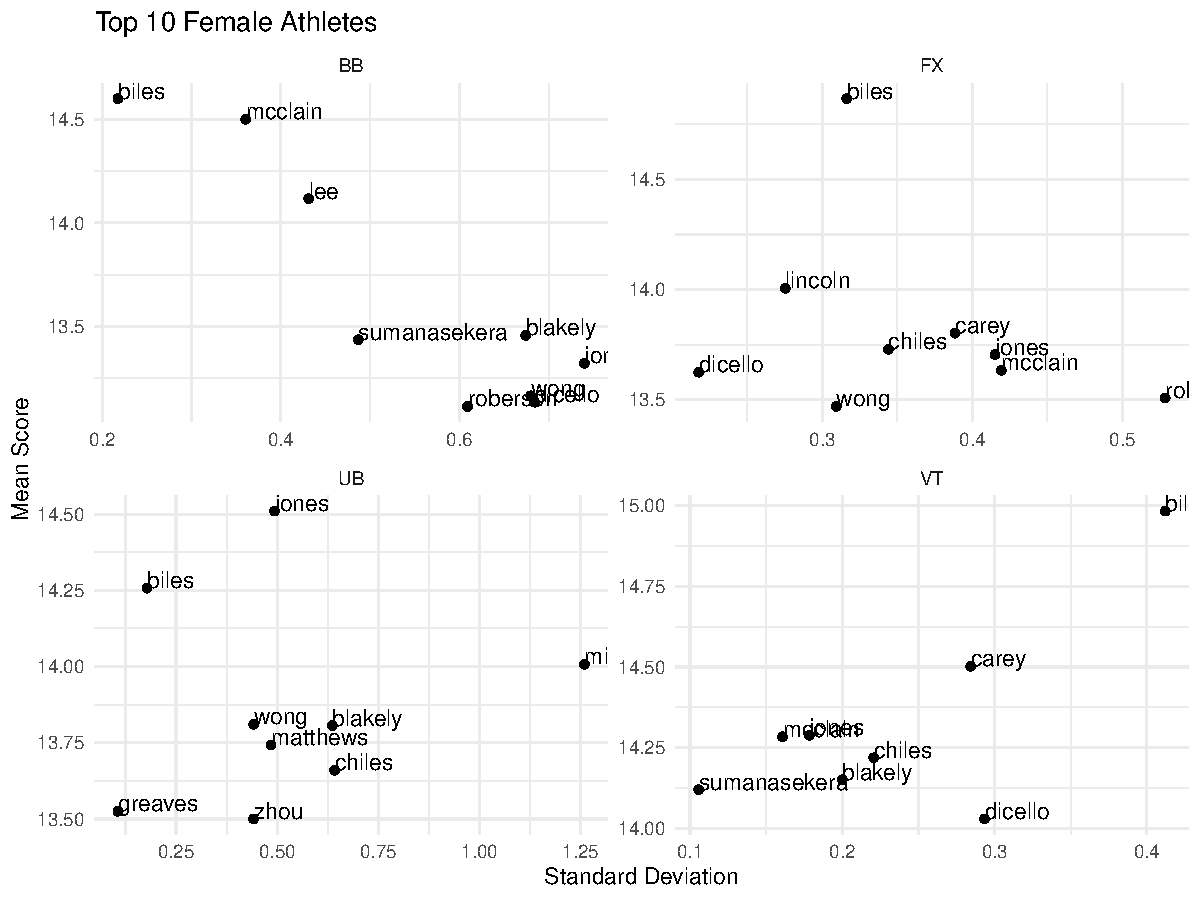
\includegraphics[scale=0.7]{FemaleAthleteApparatus.pdf}
  \caption{Top 10 Female Candidates for the Olympic Balance Beam, Floor Exercise, Uneven Bars, and Vault Apparatus}
  \label{fig:FA}
\end{figure}

\begin{table}
  \caption{Top ten female candidates for each apparatus based on mean score alone and 
  their $\mu - \alpha \sigma$ parameter values}
  \label{tab:tableBBP}
\centering
\begin{tabular}[t]{llllllll}
 \toprule
  \multicolumn{2}{c}{BB} & \multicolumn{2}{c}{FX} & \multicolumn{2}{c}{UB} & \multicolumn{2}{c}{VT}\\
  \cmidrule(lr){1-2}\cmidrule(lr){3-4}\cmidrule(lr){5-6}\cmidrule(lr){7-8}
Athlete & $\mu - \sigma$ & Athlete & $\mu - \sigma$ & Athlete & $\mu - 0.5 \sigma$ & Athlete & $\mu - 0.5 \sigma$\\
\midrule
biles & 14.38 & biles & 14.55 & jones & 14.26 & Biles & 14.78\\
\midrule
mcclain & 14.14 & lincoln & 13.73 & biles & 14.17 & Carey & 14.36\\
\midrule
lee & 13.69 & carey & 13.41 & wong & 13.59 & Mcclain & 14.20\\
\midrule
sumanasekera & 12.95 & dicello & 13.4 & matthews & 13.50 & Jones & 14.20\\
\midrule
blakely & 12.78 & chiles & 13.38 & blakely & 13.49 & Chiles & 14.11\\
\midrule
jones & 12.58 & jones & 13.29 & greaves & 13.47 & sumanasekera & 14.07\\
\midrule
roberson & 12.50 & mcclain & 13.21 & miller & 13.38 & blakely & 14.05\\
\midrule
wong & 12.48 & wong & 13.16 & chiles & 13.34 & dicello & 13.88\\
\midrule
dicello & 12.45 & roberson & 12.98 & zhou & 13.28 & richardson & NA\\
\midrule
frazier & NA & frazier & NA & walker & NA & torry & NA\\
\bottomrule
\end{tabular}
\end{table}

Based on the plot of the top ten female athletes on the balance beam apparatus I selected the parameter of 
the score standard deviation subtracted from the mean score in order to identify the best suited five 
athletes. Based on the parameter, the five ``best'' female athletes on balance beam are Biles, Mcclain, 
Lee, Sumanasekera, and Blakely.



Based on the plot of the top ten female athletes on the floor exercise apparatus I selected the parameter of 
the score standard deviation subtracted from the mean score in order to identify the best suited five 
athletes. Based on the parameter, the five ``best'' female athletes for floor exercise are Biles, Lincoln, Carey, 
Mcclain, Dicello, Chiles.



Based on the plot of the top ten female athletes on the uneven bars apparatus I selected the parameter of 
half of the score standard deviation subtracted from the mean score in order to identify the best suited five 
athletes. Based on the parameter, the five ``best'' female athletes for uneven bars are Jones, Biles, Wong, 
Matthews, and Blakely.



Based on the plot of the top ten athletes on the vault apparatus I selected the parameter of 
half of the score standard deviation subtracted from the mean score in order to identify the best suited five 
athletes. Based on the parameter, the five ``best'' female athletes on vault are Biles, Carey, Mcclain, Jones, 
and Chiles.

Ultimately, the list of athletes that ranked among the top five United States female athletes includes Biles, 
Mcclain, Lee, Sumanasekera, Blakely, Carey, Jones, Chiles, Wong, Matthews, Lincoln, and Dicello. However, Lee 
only has reported data for two out of four of the female apparatuses so she will not be considered with the other 
eleven athletes for individual or team all-around. Thus, the list of selected athletes that are involved in future 
computations includes Biles, Mcclain, Sumanasekera, Blakely, Carey, Jones, Chiles, Wong, Matthews, Lincoln, 
and Dicello.

\begin{figure}
  \centering
  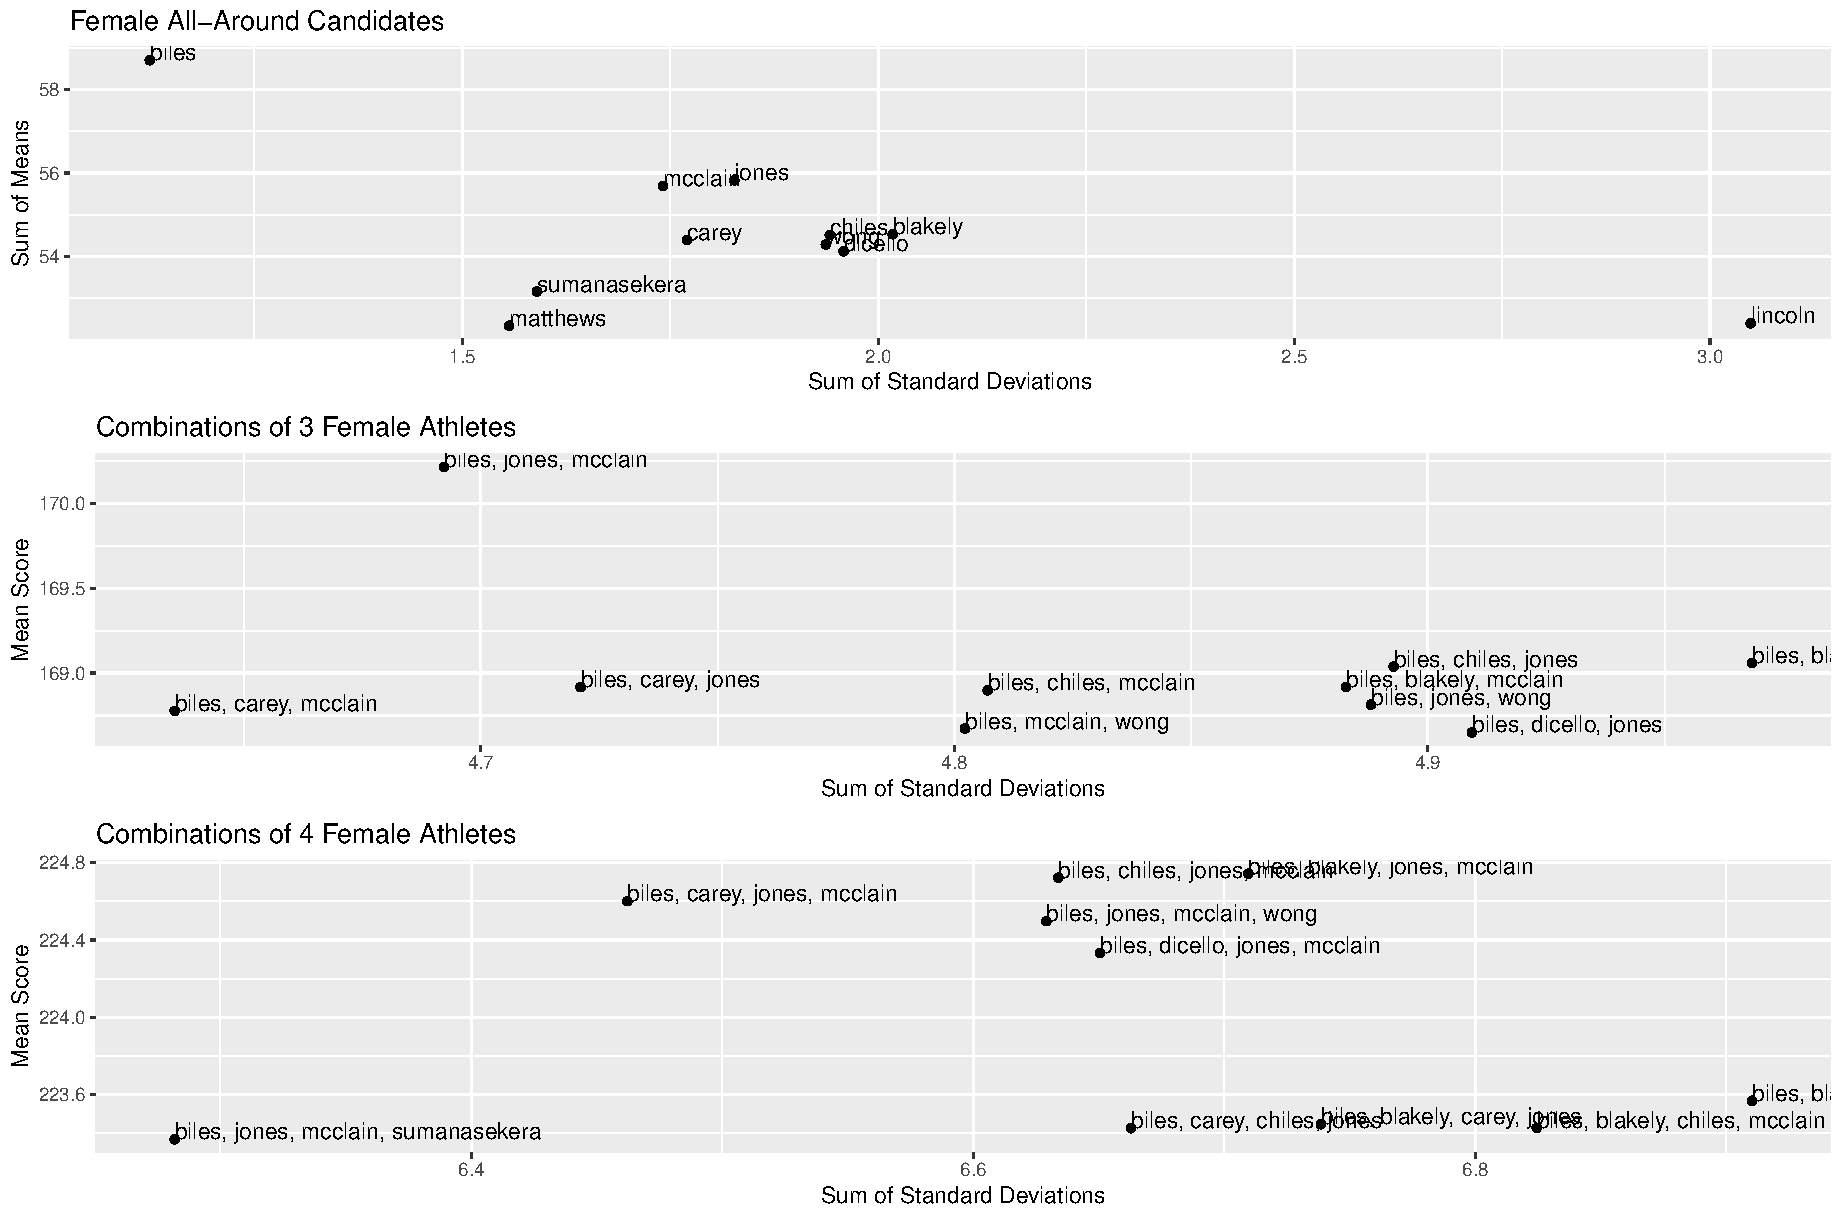
\includegraphics[scale=0.55]{FemaleMultipleAllAround.pdf}
  \caption{The best candidates for the female individual all-around and team all around medals}
  \label{fig:FAA}
\end{figure}



Figure~\ref{fig:IAA} and table~\ref{tab:tableIAA} display the summed mean score and standard deviation 
for each of the eleven selected female all-around candidates.





Figure~\ref{fig:AA3} and table~\ref{tab:tableAA3} display the summed mean score and standard deviation 
for the top combinations of three of the eleven selected female all-around candidates.



Figure~\ref{fig:AA4} and table~\ref{tab:tableAA4} display the summed mean score and standard deviation 
for the top combinations of four of the eleven selected all-around candidates.


  Based on the plot of the top ten male athletes on the floor exercise apparatus I selected the parameter of 
  the score standard deviation subtracted from the mean score in order to identify the best suited five 
  athletes. Based on the parameter, the five ``best'' male athletes on floor exercise are Juda, Mccool, Young, Moldauer, 
  and Hong.

  Based on the plot of the top ten male athletes on the vault apparatus I selected the parameter of 
  the score standard deviation subtracted from the mean score in order to identify the best suited five 
  athletes. Based on the parameter, the five ``best'' male athletes on vault are Hale, Young, Malone, Briones, and 
  Juda.

  Based on the plot of the top ten male athletes on the still rings apparatus I selected the parameter of 
  half of the score standard deviation subtracted from the mean score in order to identify the best suited five 
  athletes. Based on the parameter, the five ``best'' male athletes on still rings are Whittenburg, Briones, Diab, 
  Hong, and Loos.

  Based on the plot of the top ten male athletes on the pommel horse apparatus I selected the parameter of 
  half of the score standard deviation subtracted from the mean score in order to identify the best suited five 
  athletes. Based on the parameter, the five ``best'' male athletes on pommel horse are Nedoroscik, Young, Malone, 
  Dang, and Bock.

  Based on the plot of the top ten male athletes on the parallel bars apparatus I selected the parameter of 
  half of the score standard deviation subtracted from the mean score in order to identify the best suited five 
  athletes. Based on the parameter, the five ``best'' male athletes on parallel bars are Hong, Chou, Walker, Malone, 
  and Phillips.

  Based on the plot of the top ten male athletes on the high bar apparatus I selected the parameter of 
  half of the score standard deviation subtracted from the mean score in order to identify the best suited five 
  athletes. Based on the parameter, the five ``best'' male athletes on high bar are Malone, Juda, Briones, Bold, and 
  Nguyen.

  Ultimately, the list of athletes that ranked among the top five United States male athletes 19 distinct 
  names. However, nine of these athletes have not competed on all six apparatuses, so they will not be considered 
  with the other ten athletes for individual or team all-around. Thus, the list of selected athletes that 
  are involved in future computations includes Juda, Young, Moldauer, Hong, Hale, Malone, Whittenburg, Loos, 
  Bock, and Walker.

  Figure~\ref{fig:IAAM} displays the summed mean score and standard deviation 
  for each of the ten selected male all-around candidates.


  Figure~\ref{fig:MAA3} displays the summed mean score and standard deviation 
  for the top combinations of three of the ten selected male all-around candidates.
  

  Figure~\ref{fig:MAA4} displays the summed mean score and standard deviation 
  for the top combinations of four of the ten selected male all-around candidates.

\section{Discussion}
\label{sec:dis}

In my preliminary steps, I calculated the mean and standard deviation for every female athlete on each 
apparatus they were reported to have competed on. From these calculations, I decided to cut out most athletes 
by only inspecting athletes that ranked in the top ten by mean score alone for each apparatus. This was a 
reasonable elimination of data as the score values among the top ten candidates varied enough, often by over a 
full point, to justify that athletes that never ranked in the top ten for a particular apparatus are not 
competitive enough to medal at the Olympics.

I later developed a parameter for each apparatus to further reduce the list of athletes to only include athletes 
that rank in the top five for each apparatus. However, I designed the parameters to be dependent on the score 
standard deviation in addition to the mean score. The intent of the paramter is to create a frontier that selects 
athletes that have high mean scores and low standard deviations in order to select athletes that are the most 
successful and consistent. Ultimately, for each apparatus I selcted the five athletes with highest parameter value.

For the blanace beam apparatus, I selected the parameter: mean score minus standard deviation. This parameter 
is very reasonable as it selects athletes with high means and low standard deviations first (Biles then Mcclain 
then Lee) and selects athletes with lower standard deviations when means are similar (Sumanasekera then Blakely).

For the floor exercise apparatus, I selected the parameter: mean score minus standard deviation. This parameter 
is reasonable as well as it selects athletes with high means and low standard deviations first (Biles then Lincoln) 
and selects athletes with lower standard deviations when means are similar (Carey, Dicello, and Chiles). Note, the 
order in which Carey, Dicello, and Chiles ``should'' be selected is debatable, but it is most important that the 
parameter selected these athletes as opposed to athletes that have similar mean scores but higher standard deviations 
(Jones and Mcclain) or low standard deviations and low low mean scores (Wong).

For the uneven bars apparatus, I selected the parameter: mean score minus half of the standard deviation. 
This parameter is reasonable as well as it selects athletes with extremely high means first (Jones then Biles) and selects 
athletes with lower standard deviations when means are similar (Wong then Matthews then Blakely). 

For the vault apparatus, I selected the parameter: mean score minus half of the standard deviation. 
This parameter is reasonable as well as it selects athletes with extremely high means first (Biles then Carey) and selects 
athletes with lower standard deviations when means are similar (Mcclain then Jones then Chiles). 

Then, I used these candidates in order to determine who is best suited to compete in the all-around events. 
First, I calculted the summed mean score and summed standard deviation for each selected athlete. Looking at the data 
values and plot of these individual all-around candidates, it is very clear that Biles is strong candidate to 
compete for the individual all-around medal. However, it is not clear whether Jones or Mcclain is better suited 
to be the second United States individual all-around candidate.

Then, I used the summed mean score and summed standard deviation for each selected athlete to calculate the 
summed mean score and summed standard deviation for every combination of 
three and four of these selected athletes. Looking at the data values and plot of the combinations of three athletes, 
it is clear that Biles, Jones, and Mcclain are by far the best suited trio to compete for the team all-around medal. 
Additionally, since this data suggests that both Mcclain and Jones should compete in the qualifying round, there 
is no need to select one over the other for the second individual all-around candidate spot as they would both get 
the opportunity to qualify, and their scores at the Olympics will determine which athlete, if either, will qualify 
to attend the individual all-around finals. 

Looking at the data values and plot of the combinations of four athletes, it is not clear whether Chiles, Carey, or 
Blakely is best suited to be the fourth team all-around candidate as their means and standard deviations are very 
similar. However, looking at the individual apparatus events provides justification for who to ultimately select. 
Knowing that two athletes per country can compete for an apparatus medal, it is strategic to try to compose the 
team of the best two United States athletes for each apparatus. Based on the computations and plots, the superior two 
athletes on balance beam are Biles and Mcclain, the superior two athletes on floor exercise are Biles and Lincoln, 
the superior two athletes on uneven bars are Jones and Biles, and the superior two athletes on vault are Biles 
and Carey. Since Lincoln was not among our top candidates for an all-around medal, it would be logical to select her 
as the fifth United States Olympic team member who does not compete in the all-around qualifying round. Additionally, 
since Carey is one of the candidates being considering for the all-around qualifying round and she is one of our superior 
athletes on vault, it is reasonable to also select her to be the final member of the Olympic team. Although, the 
summed combination that included Carey has the lowest mean in comparison to the combinations including Chiles or 
Blakely, the selection of Carey can be further justified by the facts that the summed mean score difference is 
within one point the combination including Carey has the lowest summed standard deviation.

Ultimately, in order to maximize the the number of medals the Unites States female team wins, I would comprise the 
team of the athletes Biles, Jones, Mcclain, Lincoln, and Carey.

\appendix

\section{Appendix: Application of the Mean and Standard Deviation Derived Parameters Methods For The Male 
United States Artistic Gymnastics Team at The 2024 Paris Olympics}

\begin{figure}
  \centering
  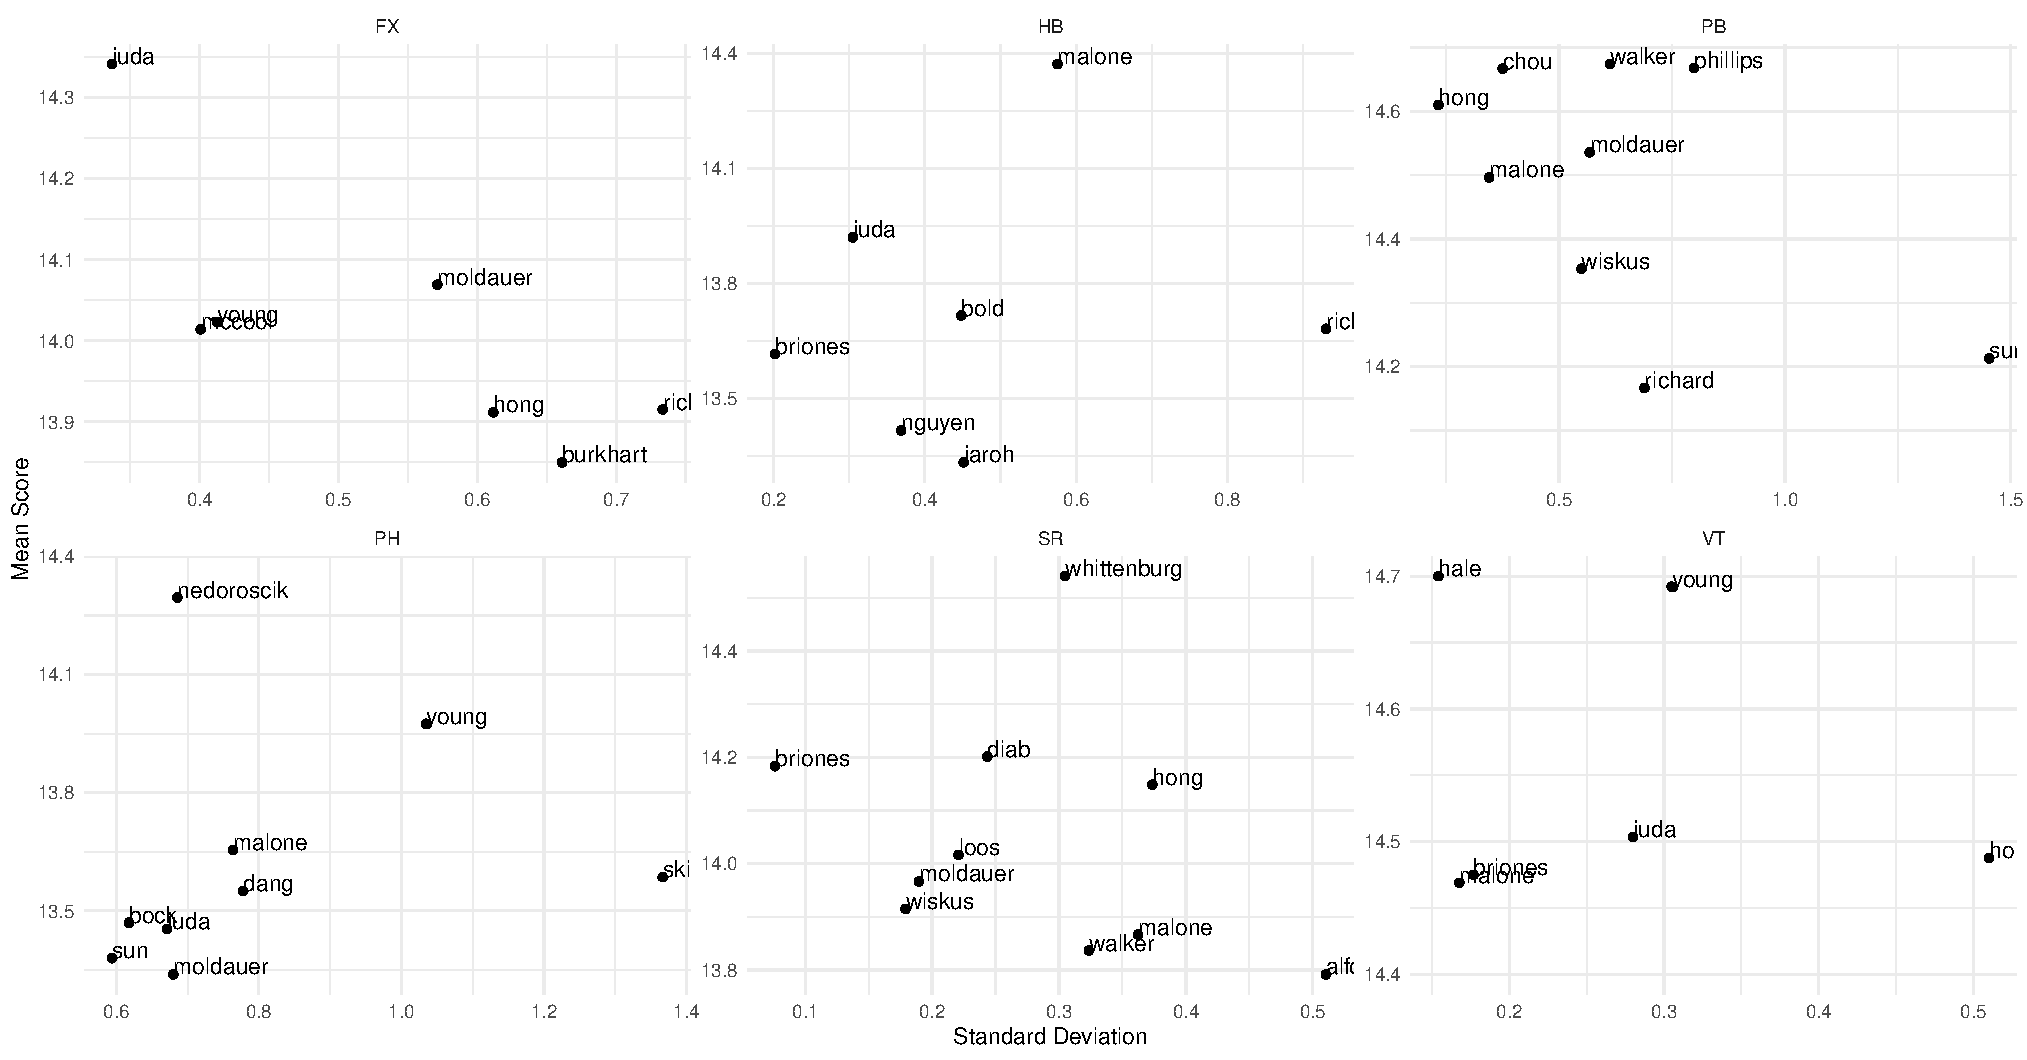
\includegraphics[scale=0.5]{MaleAthleteApparatus.pdf}
  \caption{Top 10 Male Candidates for the Olympic Floor Exercise, Pommel Horse, Still Rings, Vault, Parallel Bars, 
  and High Bar Apparatus}
  \label{fig:FA}
\end{figure}

\begin{figure}
  \centering
  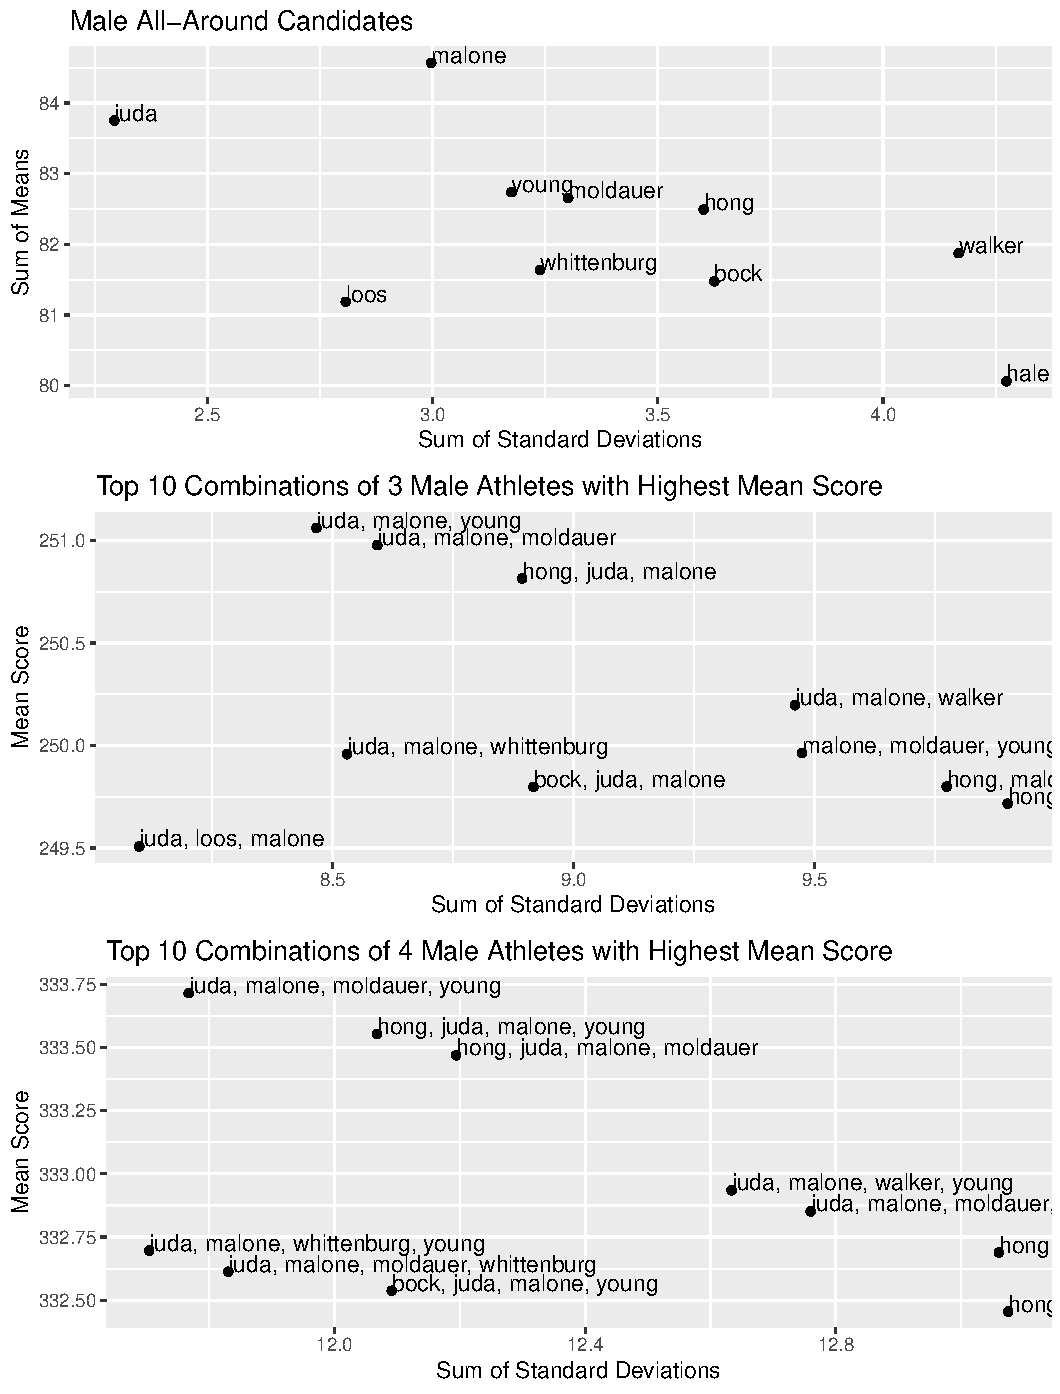
\includegraphics[scale=0.7]{MaleMultipleAllAround.pdf}
  \caption{The best candidates for the male individual all-around and team all around medals}
  \label{fig:FAA}
\end{figure}


For men, the overall statistical method I used to determine the team of five male gymnasts that should be sent 
to the 2024 Olympics was very similar, but varied when it came to determining the final fifth team member. After 
using the same method to determine the United States' best four male candidates for the team all-around qualification 
round, I calculated the mean score for every male gymnast on every apparatus in order to determine which apparatuses 
the male USA team had the greatest chance of earning medals on. From this data, there was only one additional male 
USA gymnast that ranked globally in the top ten for a particular apparatus based on mean score alone.

When determining the most ideal American male candidates, 
I did inspect the data of non United States gymnasts in order to determine which medals the United States 
male team has the greatest chance of earning. 

Similar to the female model, I used the same method to determine the ``best'' male all-around candidates as I did for females. From 
Figure~\ref{fig:IAAM} I determined that Juda and Malone are the best male Individual all-around candidates. From 
Figure~\ref{fig:MAA3} I determined that Juda, Malone, and Young are the best male team all-around finalists 
candidates. Additionally, from Figure~\ref{fig:MAA4} I determined that Moldauer is the best candidate to also compete 
with Juda, Malone, and Young in the all-around qualifying round. Comparatively, determining the ``best'' fifth Olympic 
teammate is challenging as there are several apparatuses where our ``best'' competitor is not among the four 
previously selected teammates. However, through examining the the mean score for every male gymnast on every apparatus 
we can see that many of our ``best'' candidates are still ranked very poorly globally, and therefore would not have a 
strong liklihood of medalling at the olympics. Among all of the male USA athletes that are not yet selected, the only 
athlete that has a relatively decent chance of medaling is Hale, who ranks 6th globally for the Vault apparatus.

Ultimately, in order to maximize the the number of medals the Unites States male team wins, I would comprise the 
team of the athletes Juda, Malone, Young, Moldauer, and Hale.

\bibliographystyle{chicago}
\bibliography{citations}

\end{document}